%% abtex2-modelo-include-comandos.tex, v-1.9.6 laurocesar
%% Copyright 2012-2016 by abnTeX2 group at http://www.abntex.net.br/ 
%%
%% This work may be distributed and/or modified under the
%% conditions of the LaTeX Project Public License, either version 1.3
%% of this license or (at your option) any later version.
%% The latest version of this license is in
%%   http://www.latex-project.org/lppl.txt
%% and version 1.3 or later is part of all distributions of LaTeX
%% version 2005/12/01 or later.
%%
%% This work has the LPPL maintenance status `maintained'.
%% 
%% The Current Maintainer of this work is the abnTeX2 team, led
%% by Lauro César Araujo. Further information are available on 
%% http://www.abntex.net.br/
%%
%% This work consists of the files abntex2-modelo-include-comandos.tex
%% and abntex2-modelo-img-marca.pdf
%%

% ---
% Este capítulo, utilizado por diferentes exemplos do abnTeX2, ilustra o uso de
% comandos do abnTeX2 e de LaTeX.
% ---

\chapter{Introdução}
\label{intro}
% ----------------------------------------------------------

Este documento e seu código-fonte são exemplos de referência de uso da classe \textsf{abntex2} e do pacote \textsf{abntex2cite}. O documento exemplifica a elaboração de trabalho acadêmico (tese, dissertação e outros do gênero) produzido conforme a ABNT NBR 14724:2011 \emph{Informação e documentação Trabalhos acadêmicos - Apresentação}.

A expressão ``Modelo Canônico'' é utilizada para indicar que \abnTeX\ não é modelo específico de nenhuma universidade ou instituição, mas que implementa tão somente os requisitos das normas da ABNT. Uma lista completa das normas observadas pelo \abnTeX\ é apresentada em \citeonline{abntex2classe}.

Sinta-se convidado a participar do projeto \abnTeX! Acesse o site do projeto em \url{http://www.abntex.net.br/}. Também fique livre para conhecer, estudar, alterar e redistribuir o trabalho do \abnTeX, desde que os arquivos modificados tenham seus nomes alterados e que os créditos sejam dados aos autores originais, nos termos da ``The \LaTeX\ Project Public License''\footnote{\url{http://www.latex-project.org/lppl.txt}}.

Encorajamos que sejam realizadas customizações específicas deste exemplo para universidades e outras instituições --- como capas, folha de aprovação, etc. Porém, recomendamos que ao invés de se alterar diretamente os arquivos do \abnTeX, distribua-se arquivos com as respectivas customizações. Isso permite que futuras versões do \abnTeX~não se tornem automaticamente incompatíveis com as customizações promovidas. Consulte \citeonline{abntex2-wiki-como-customizar} para mais informações.

Este documento deve ser utilizado como complemento dos manuais do \abnTeX\ \cite{abntex2classe,abntex2cite,abntex2cite-alf} e da classe \textsf{memoir} \cite{memoir}. 

Esperamos, sinceramente, que o \abnTeX\ aprimore a qualidade do trabalho que você produzirá, de modo que o principal esforço seja concentrado no principal: na contribuição científica.

Equipe \abnTeX 

Lauro César Araujo

	\section{Adição de figuras}
	
	A \autoref{intro:exemplo} apresenta um exemplo de figura criada em formato vetorial. Sempre prefira esse tipo de formato, pois ele apresenta maior qualidade tanto no formato digital quanto no formato impresso. Além disso, em geral ele gera arquivos muito mais leves, o que facilita a execução, armazenamento e transmissão da tese. Para gráficos muito complexos criados em Python, é recomendado utilizar a opção de rasterização para tornar a compilação do arquivo mais rápida. Mais detalhes podem ser encontrados em \url{https://matplotlib.org/stable/gallery/misc/rasterization_demo.html}.
		
	\begin{figure}[!h]
		\centering
		\caption{Exemplo de figura. As figuras devem ser criadas em formato PDF ou SVG sempre que possível. Quando não for possível, devem ser geradas em formato png com DPI superior a 600.}
		\label{intro:exemplo}
		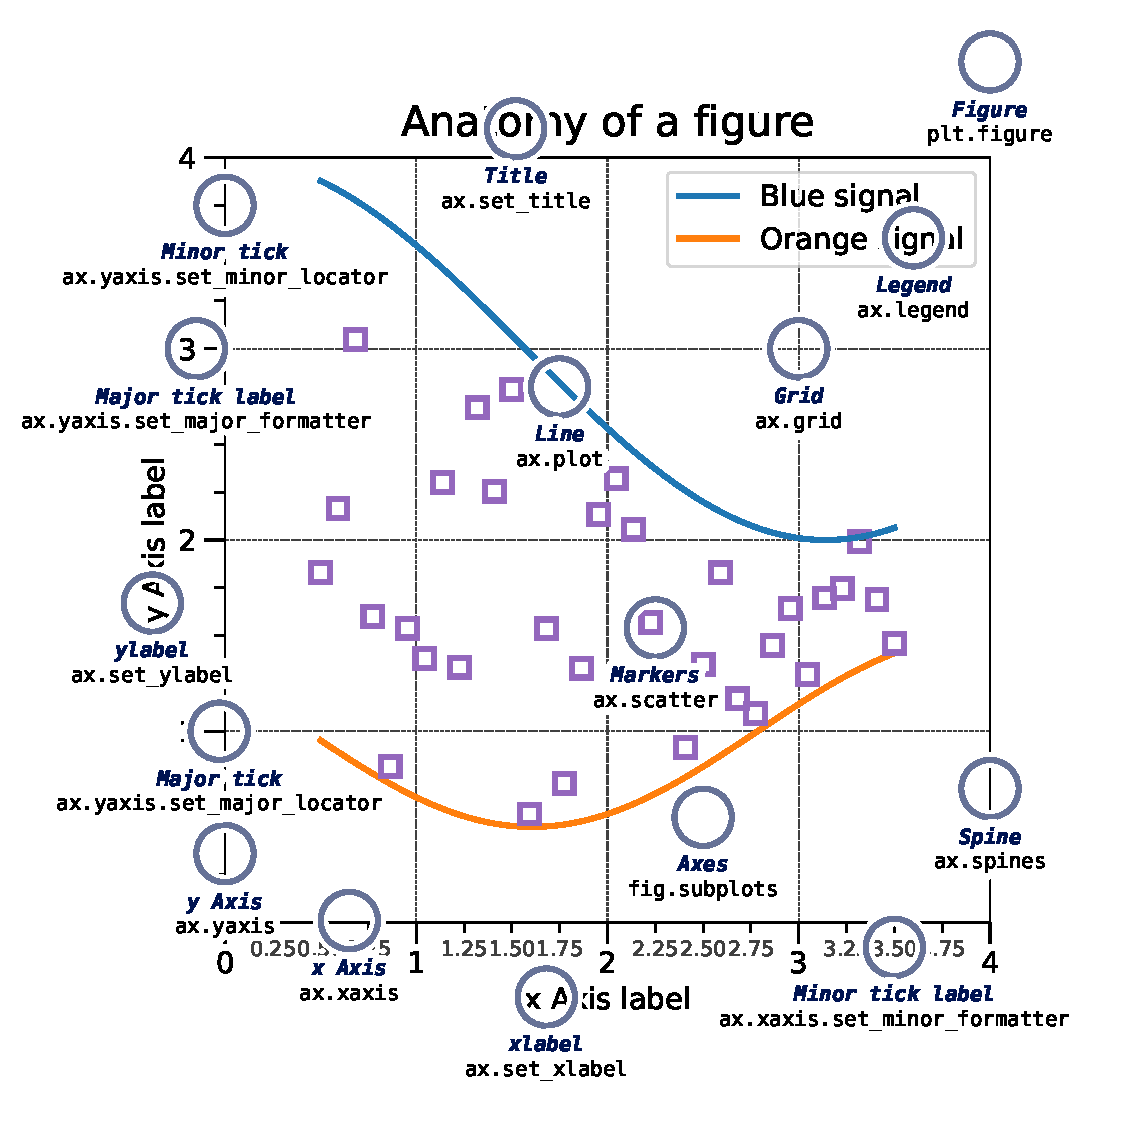
\includegraphics[width=0.8\linewidth]{capitulos/figuras/intro/figure_intro}
		\fonte{O autor.}
	\end{figure}
	
	A regra diz que a legenda fica sempre antes da figura, e a fonte após. Quando a figura for retirada de algum lugar, a fonte deve ser alterada para o padrão Autor, Ano. Ex.: Oliveira \textit{et al}, 2024
	
	


			